\documentclass[../DefinizioneDiProdotto_v3.0.0.tex]{subfiles}

\begin{document}

\section{Descrizione architetturale}

\subsection{Architettura generale}
\subsubsection{Schema architettura generale}
\begin{figure}[!h]
	\centering
	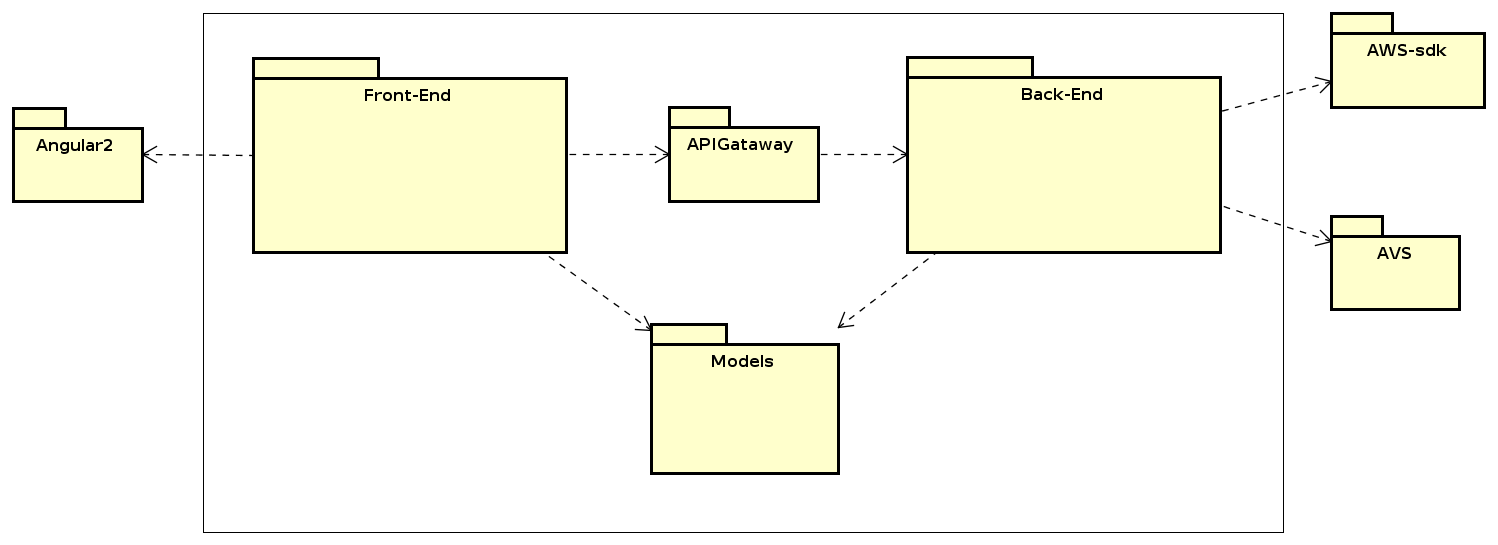
\includegraphics[width=\textwidth]{Architettura/AltoLivello.png}
	\caption{Schema architettura generale}
\end{figure}

\subsubsection{Descrizione}
Nell'esposizione dell'architettura dell'applicazione si procederà con un approccio \gl{top-down}, descrivendola dal generico al particolare. Si inizia quindi dalla descrizione dei package e dei componenti, per poi descrivere nel dettaglio le singole classi, specificando per ognuna il tipo, l'obiettivo, la funzione, relazioni in ingresso e uscita e i metodi e attributi contenuti. Successivamente verranno riportati i diagrammi di sequenza da quelli più generali a quelli delle singole chiamate API, il tutto seguendo il formalismo del linguaggio UML 2.0.

\subsubsection{Suddivisione logica}
Durante la progettazione si è deciso di adattare diversi \gl{design pattern architetturali},
difatti secondo le nostre esigenze, non era possibile adottarne uno univoco per l'intera architettura.
Il sistema è quindi stato suddiviso in due parti:
\begin{itemize}
	\item \textbf{Front-end}: la parte client del sistema, che deve essere eseguita da un qualsiasi browser, e verrà sviluppata con l'uso di AngularJS.
	\item \textbf{Back-end}: la parte risiedente nei sistemi cloud di Amazon, che eseguono l'elaborazione e forniscono i dati che verrà invece sviluppata in NodeJS e sfruttando i servizi distribuiti Amazon Web Service.
\end{itemize}
La comunicazione tra le due parti, sarà quindi gestita da un applicativo Amazon chiamato AWS APIGateway. Quest'ultimo però sarà rappresentato senza però una precisa implementazione vista la sua necessita di essere configurato tramite SWAGGER.
È stata implementata una separazione tra GuestHome e i suoi Services, e la parte di amministrazione con i relativi Services. Lo stesso è stato fatto per la parte del Back-End. Ad esempio, il package del back-end LambdaSkill contiene tutti i moduli relativi alla comunicazione con l'ospite che hanno in comune solo i moduli che contengono le specifiche dei singoli oggetti.

\subsection{Design pattern}

\subsubsection{Strutturali}

\paragraph{MVC AngularJS}\mbox{}
\begin{addmargin}[1em]{2em}% 1em left, 2em right
	\textbf{Struttura}: il Model è il livello più basso del pattern ed è responsabile della gestione dei dati utili all'applicazione.
	La View si occupa di permettere all'utente la visualizzazione delle informazioni presenti nel Model.
	Il Controller invece si occupa del controllo degli eventi inviati dalla view e modifica il model in base agli eventi stessi, mentre per reperire i dati alla rete, il controller si affiderà ad un apposito model.
	Model view e controller, vanno a formare un componente, che collegato ad una rispettiva direttiva, potrà essere richiamato all'interno di altri componenti, o, tramite router, il componente che si occupa di gestire l'indirizzamento.
	Il Service invece ha la responsabilità di gestire la chiamata alle API, e di gestire quindi le chiamate asincrone alla rete.\\
	\textbf{Utilizzo}: Questo pattern viene impiegato nello sviluppo della parte front end del progetto, e viene implementato con il framework AngularJS nella versione 2.\\
	\textbf{Motivo}: Questa scelta è stata dettata dall'impiego di AngularJS per la realizzazione del front-end, della console amministrativa e della schermata per l'ospite, che, utilizzando un pattern MVC, ha influenzato la nostra decisione. Altre motivazioni sono state l'utilizzo delle REST API e la possibilità di sfruttare gli oggetti da parte di AngularJS nella versione NodeJS da noi utilizzata, in questo modo è possibile trattare, mediante interfaccia REST, lo stesso oggetto che fa da Model, come oggetto nella parte di back-end. Il Controller si interfaccia verso le API da un'apposita classe chiamata Service.\\
	Per facilitare la comprensione di quanto appena descritto, viene fornito una schema riportante la struttura MVC adottata.
\end{addmargin}
\clearpage
\begin{figure}[!h]
	\centering
	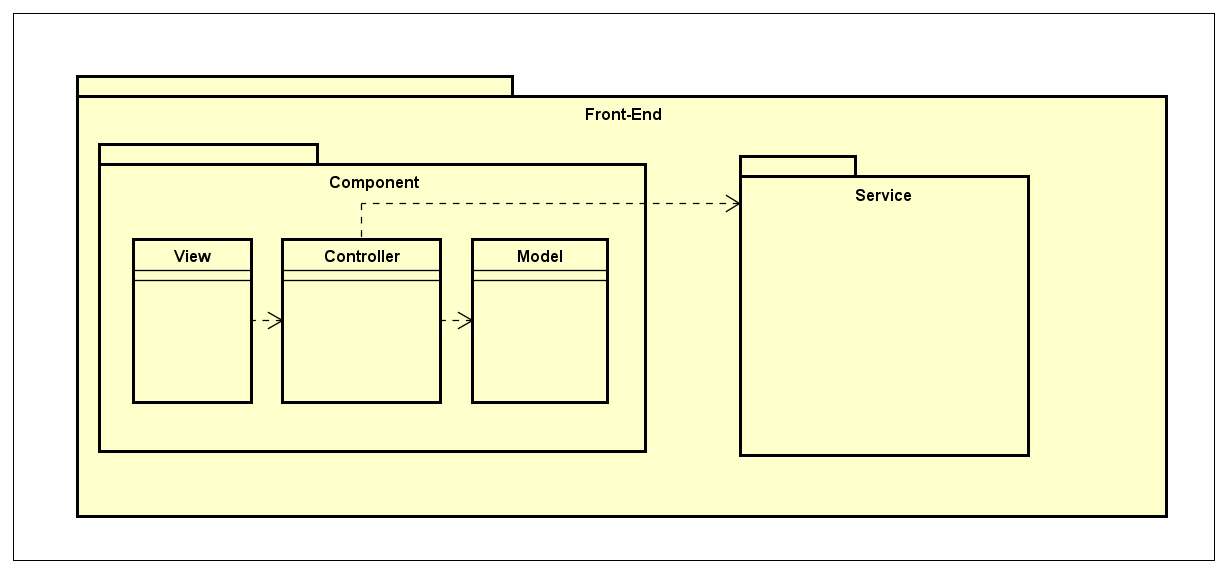
\includegraphics[width=\textwidth]{Architettura/MVC.png}
	\caption{Schema MVC}
\end{figure}

\paragraph{Handler-Module Pattern}\mbox{}
\begin{addmargin}[1em]{2em}% 1em left, 2em right
	\textbf{Struttura}:	L'APIGateway alla chiamata di una risorsa, rilascia un evento contenente tutte le informazioni della chiamata. Questo verrà gestito da un'apposita funzione che avrà lo scopo di scegliere l'opportuna funzionalità del service associato, prima della chiamata al servizio, verrà controllata anche la compatibilità di tipo.\\
	\textbf{Utilizzo}:  Questo pattern viene impiegato per lo sviluppo dei service, che verranno utilizzati sia per la parte amministrativa che per la parte guest.\\
	\textbf{Motivo}: Questo pattern viene usato per la parte amministrativa, allo scopo di ridurre l'accoppiamento tra chi offre i servizi e chi invece gestisce l'evento di handling. L'alternativa Amazon sarebbe stata di produrre una funzione per ogni risorsa, ma con la caratteristica di diventare molto complessa e eccessivamente decentralizzata.
\end{addmargin}

\paragraph{REST API}\mbox{}
\begin{addmargin}[1em]{2em}% 1em left, 2em right
	\textbf{Struttura}: REST API (REpresentational State Transfer Application Programming Interface) consiste in sei vincoli da rispettare:
	\begin{itemize}
		\item \textbf{Client-Server}: richiede la separazione tra l'interfaccia utente dai dati da archiviare, così da migliorare la portabilità dell'interfaccia tra diverse piattaforme e la scalabilità, semplificando i componenti server. Così facendo si possono sviluppare le componenti indipendentemente;
		\item \textbf{Stateless}: la comunicazione client-server è vincolata dall'assenza di una memorizzazione, nel server, del contesto. Ogni chiamata, non possiede nessuna memoria delle precedenti avvenute, questo non implica però che, al di fuori della chiamata, ci siano dei token di riconoscimento appositi;
		\item \textbf{Cacheable}:  i client possono fare \gl{caching} delle risposte. Le risposte devono in ogni modo definirsi implicitamente o esplicitamente cacheable o no, in modo da evitare che i client possano riusare stati datati o dati errati. Una gestione ben fatta della cache può ridurre, o addirittura parzialmente eliminare, le comunicazioni client-server, migliorando scalabilità e performance;
		\item \textbf{Layered system}: un client non può dire se è connesso direttamente ad un server di livello più basso o intermedio. I server intermedi possono migliorare la scalabilità del sistema con il \gl{load-balancing} o con le \gl{cache distribuite}. Possono esserci dei \gl{layer} intermedi per offrire la configurazione di politiche di sicurezza;
		\item \textbf{Code on demand}:  i server possono temporaneamente estendere o personalizzare le funzionalità del client trasferendo del codice eseguibile. Ad esempio questo può includere componenti compilate come \gl{Applet Java} o linguaggi di scripting client-side come JavaScript. "Code on demand" è l'unico vincolo opzionale per la definizione di un'architettura REST;
		\item \textbf{Uniform interface}: un'interfaccia di comunicazione omogenea tra client e server che permette di semplificare e disaccoppiare l'architettura, la quale si può evolvere separatamente.
	\end{itemize}.\\
	\textbf{Utilizzo}: viene utilizzato nell'interfaccia tra Front-End e Back-End.\\
	\textbf{Motivo}: questa scelta è dovuta alla larga diffusione di questo metodo per la gestione di chiamate HTTP/HTTPS, che lo rende ormai standard, e per la semplicità di implementazione con il meccanismo Lambda di Amazon che ne fornisce un apposito servizio (AWS APIGateway) concepito per interfacciarsi con \gl{SWAGGER}.

\end{addmargin}
\begin{figure}[!h]
	\centering
	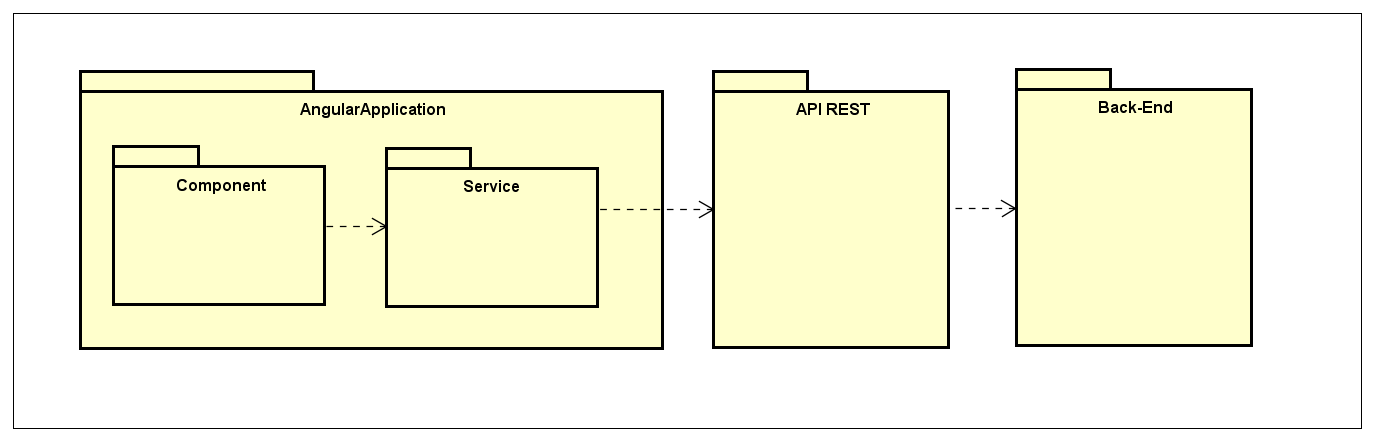
\includegraphics[width=\textwidth]{Architettura/API-Rest.png}
	\caption{Schema REST API}
\end{figure}

\subsubsection{Comportamentali}
Viene adottato un solo \gl{design pattern comportamentale} nell'architettura, l'Observer, per sincronizzare i vari oggetti dipendenti tra loro.

\paragraph{Observable http request}\mbox{}
\begin{addmargin}[1em]{2em}% 1em left, 2em right
	\textbf{Struttura}: Il funzionamento di questo pattern utilizzato in AngularJS ha un funzionamento simile alle promise.
	La funzione che si interfaccia alla rete, ritorna un oggetto chiamato "Observable", che funge da "Stub" che dovrà contenere il risultato dell'operazione, che viene svolta in asincronia.
	Tutti i rifermenti a quell'oggetto, saranno quindi in attesa del risultato. Quando la richiesta viene soddisfatta, tutte le operazioni in attesa verranno soddisfatte.  \\
	\textbf{Utilizzo}: viene utilizzato per la conversazione tra i \gl{services} e i \gl{component} del Front-End, utilizzando il framework AngularJS.\\
	\textbf{Motivo}: Utilizzando questo pattern, il codice diventa più chiaro, e l'operazione viene svolta in completa asincronia, riducendo la dipendenza tra service e component, migliorando l'efficienza e riducendo la complessità nel seguire il flusso.
\end{addmargin}

\paragraph{Promise pattern}\mbox{}
\begin{addmargin}[1em]{2em}% 1em left, 2em right
	\textbf{Struttura}: Le funzioni da eseguire asincronamente, vengono accorpate dentro a degli oggetti chiamati promise. I metodi done() e fail() di una promise consentono di specificare cosa fare dopo aver ottenuto il risultato positivo o negativo dell’elaborazione asincrona. Questi stessi metodi restituiscono delle promise, così possiamo concatenare più done() per mettere in sequenza operazioni asincrone in maniera più leggibile delle callback annidate.\\
	\textbf{Utilizzo}: Viene utilizzato nella parte di servizi lambda,più in particolare nella parte richiamata da Alexa (Alexa Skill), nel supporto alla programmazione asincrona, cioè alla possibilità di eseguire attività in background che non interferiscono con il flusso di elaborazione principale.\\
	\textbf{Motivo}: Nello sviluppo di funzioni con contesti asincroni, è necessario rendere rapido e più chiaro il flusso del programma, nel caso ci sia un numero consistente di chiamate successive alla conversazione. Questo ripiazza di fatto il patterna callback, ove è presente.\\
\end{addmargin}

\paragraph{Callback pattern}\mbox{}
\begin{addmargin}[1em]{2em}% 1em left, 2em right
	\textbf{Struttura}: Le funzioni da eseguire asincronamente, ottengono come parametro una funzione chiamata "callback" che viene chiamata una volta e una sola volta. Si chiama quando si verifica un errore, o quando il risultato è disponibile; Questa funzione accetta due argomenti ed hanno valori diversi a seconda che si è verificato un errore o meno:\\
		Se si è verificato nessun errore:
		Il primo argomento callback è nullo o non definito ed il secondo argomento contiene i risultati di richiamata.\\
		In caso di errore:
		il primo argomento contiene un oggetto errore, mentre il secondo argomento sarà indefinito. \\
	\textbf{Utilizzo}: Viene utilizzato nella parte di servizi ed API, nel supporto alla programmazione asincrona, cioè alla possibilità di eseguire attività in background che non interferiscono con il flusso di elaborazione principale. In particolare questo pattern viene utilizzato in tutte le funzione che dialogando con il database e quindi la class DatabaseInteraction, deve essere svolte forzatamente in asincronia.\\
	\textbf{Motivo}: Nello sviluppo di funzioni con contesti asincroni, è  necessario effettuare una funzione successivamente, dopo aver avuto il risultato della funzione chiamata. In javascript questo avviene chiamando la funzione di ritorno all'interno di quella chiamata.\\
\end{addmargin}

\subsection{Descrizione architetturale}
\subsubsection{Architettura Front-end}
\begin{figure}[!h]
	\centering
	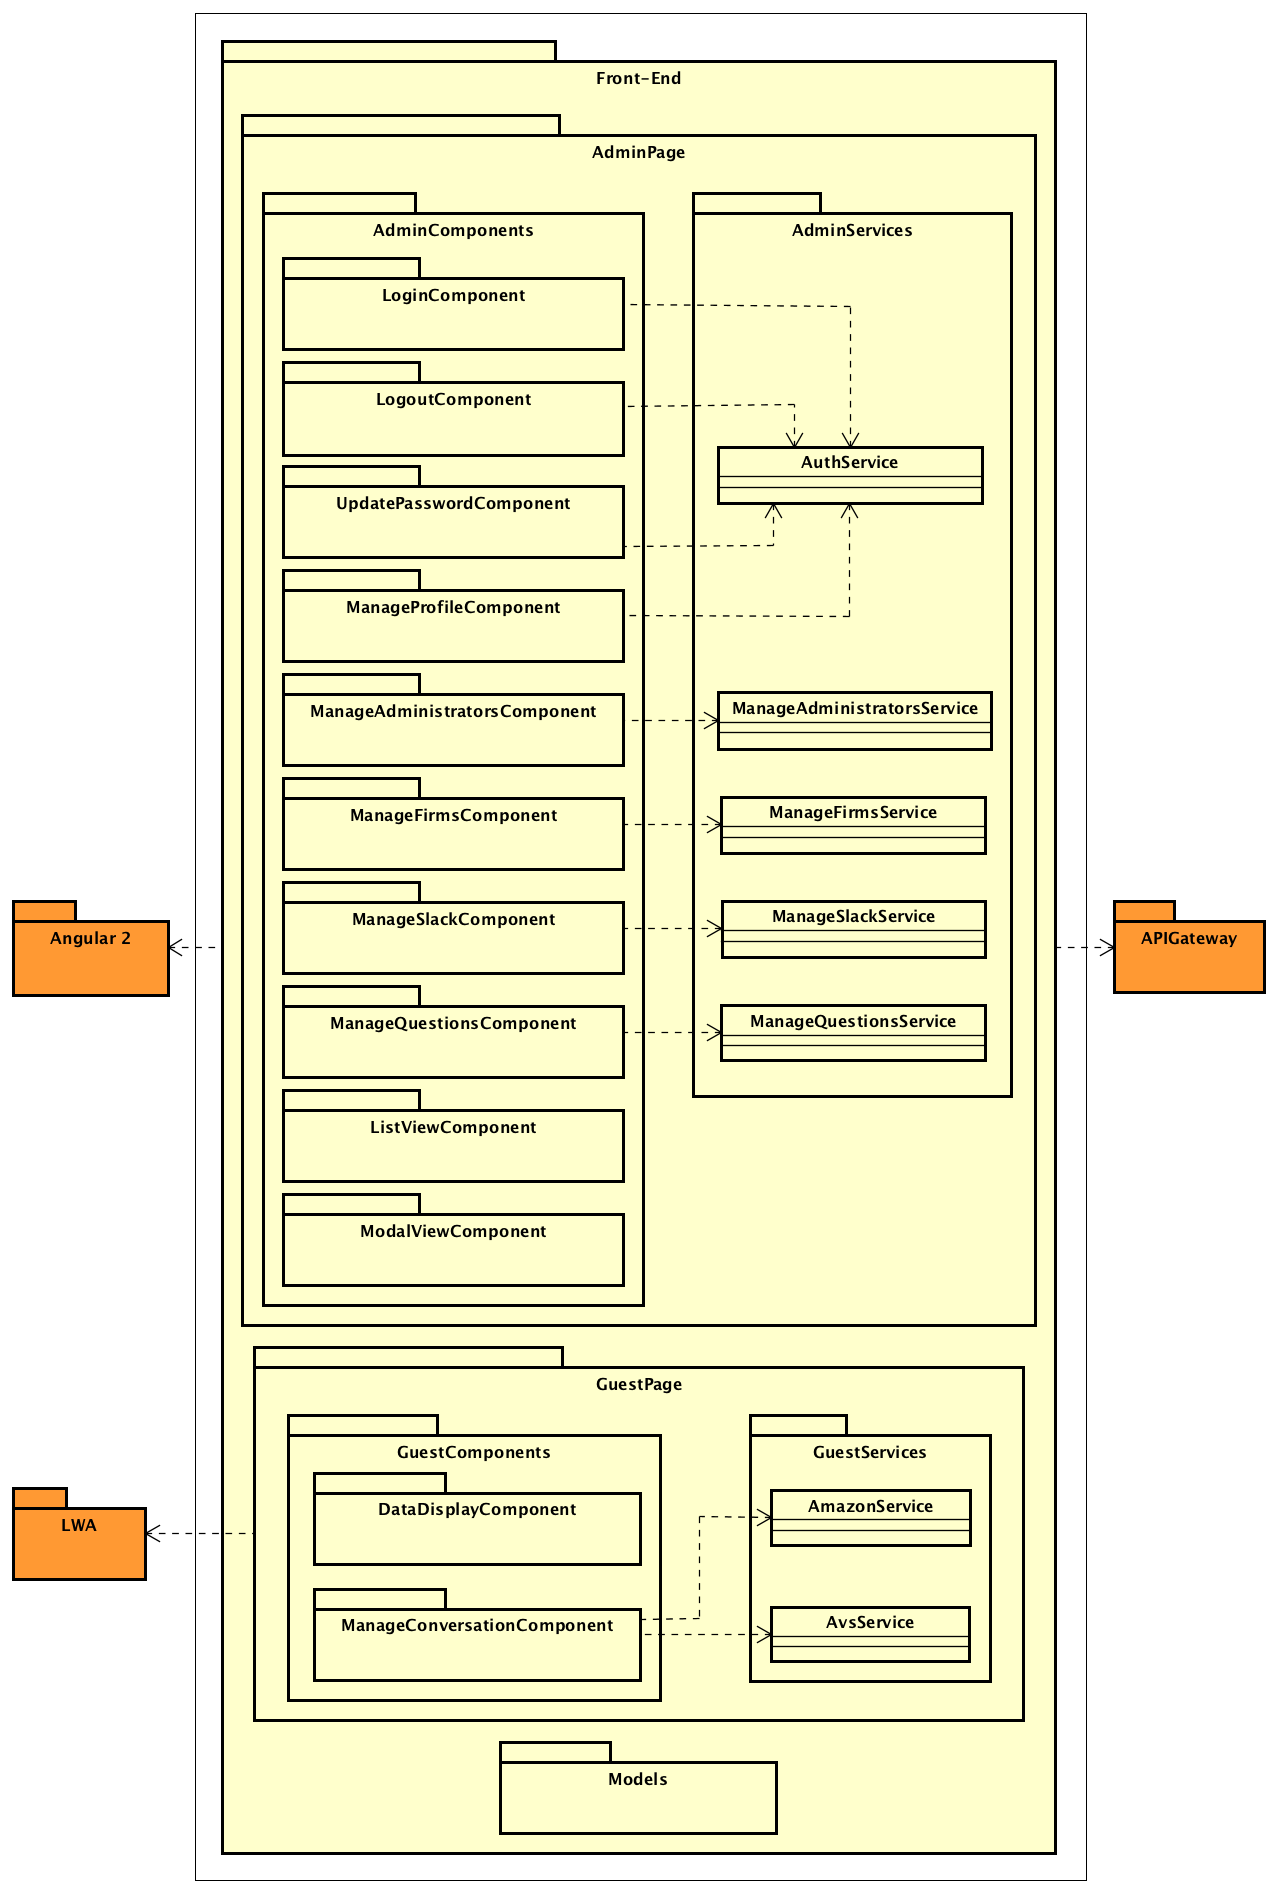
\includegraphics[scale=0.45]{Architettura/Front-end.png}
	\caption{Schema architettura Front-End}
\end{figure}

\subparagraph{Descrizione}	La parte del Front-End è sviluppata in AngularJS e ne rispecchia il pattern di sviluppo: ogni componente (ogni package rappresenta un Model-View-Controller) è immerso nella pagina. Di seguito è disponibile una lista delle \gl{route} delle pagine per i relativi tracciamenti per comprendere al meglio quando i vari componenti vengono attivati. \\

\begin{longtable}[c] { >{\centering\arraybackslash}p{5cm} >{\centering\arraybackslash}p{5cm} }
	\toprule
	{\textbf{Componente}} & {\textbf{Route}}       \\
	\midrule
	Login                 & /admin/login           \\
	\addlinespace[0.3em]
	\midrule
	UpdatePassword        & /admin/updatePassword  \\
	\addlinespace[0.3em]
	\midrule
	ManageGuests          & /admin/manageGuest     \\
	\addlinespace[0.3em]
	\midrule
	ManageAdministrators  & /admin/manageAdmins    \\
	\addlinespace[0.3em]
	\midrule
	ManageSlack           & /admin/manageSlack     \\
	\addlinespace[0.3em]
	\midrule
	ManageQuestions       & /admin/manageQuestions \\
	\addlinespace[0.3em]
	\midrule
	ManageProfile         & /admin/manageProfile   \\
	\addlinespace[0.3em]
	\midrule
	StartStop             & /guestHome             \\
	\addlinespace[0.3em]
	\midrule
	DataDisplay           & /guestHome             \\
	\addlinespace[0.3em]
	\midrule
	Conversation          & /guestHome             \\
	\addlinespace[0.3em]
	\bottomrule
	\caption{Tracciamento Component-Route AngularJS}
\end{longtable}

\clearpage

Il Front-End ha anche il compito di gestire la comunicazione con AVS per dialogare con Alexa. A tal scopo, prima di poter usare l'applicazione, dopo l'apertura, viene effettuato il Login With Amazon (LWA). Quest'operazione avviene in due fasi, la richiesta del code a LWA, e la richiesta del CodeToken alle API del back-end, che confermeranno l'autenticazione. Sarà inoltre prevista una richiesta alle API per il refresh del token dopo la scadenza.

\begin{figure}[!h]
	\centering
	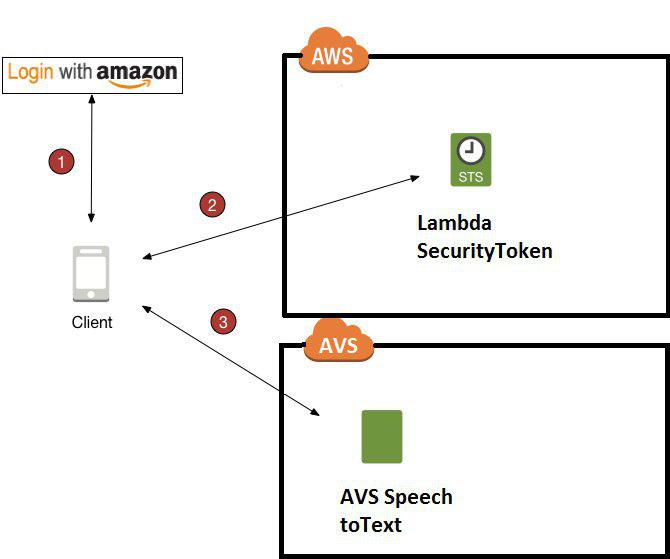
\includegraphics[scale=0.5]{Architettura/schemaAutenticazione.jpg}
	\caption{Schema funzionamento Login With Amazon}
\end{figure}

\clearpage
\subsubsection{Architettura Back-End}
\begin{figure}[!h]
	\centering
	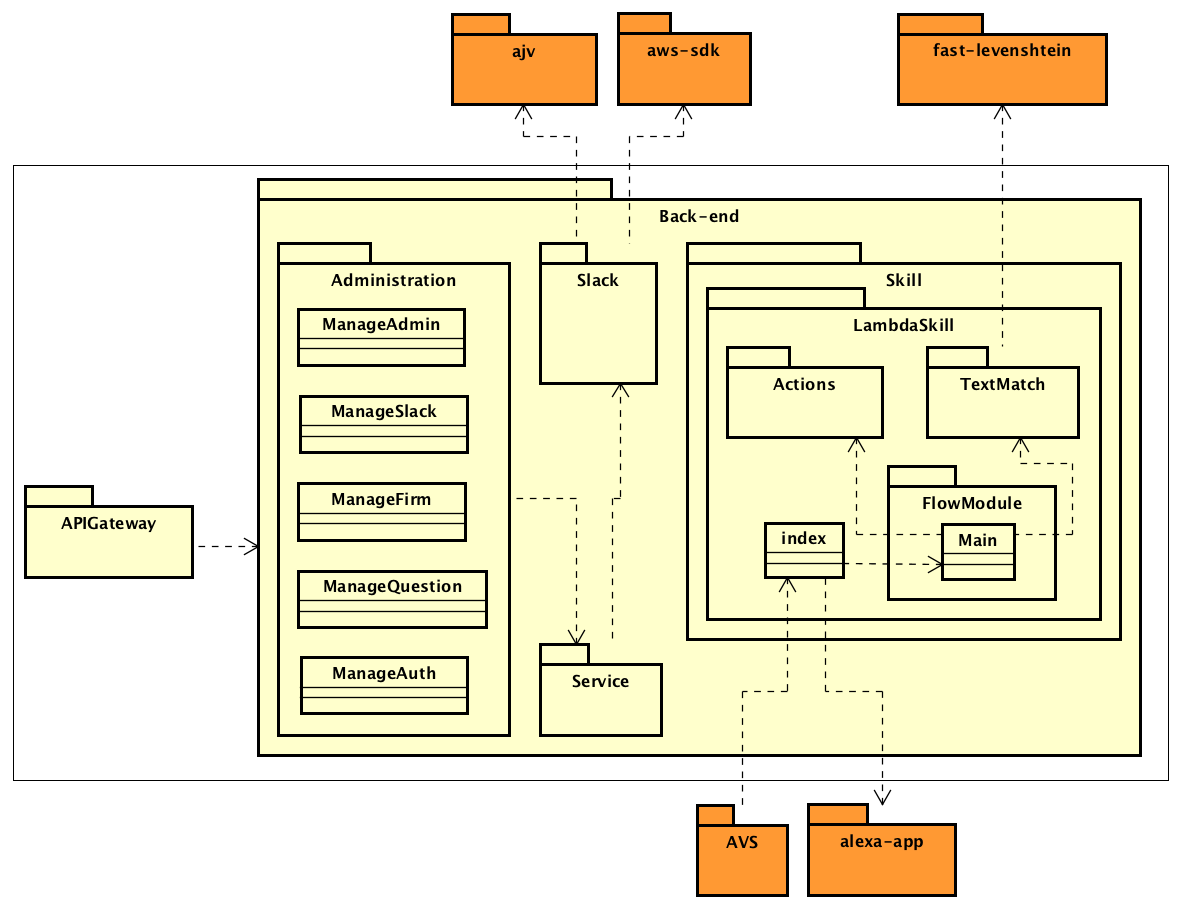
\includegraphics[scale=0.5]{Architettura/Back-end.png}
	\caption{Schema architettura Back-End}
\end{figure}

\subparagraph{Descrizione}
Nel Back-End sono state progettate separatamente le componenti che interagiscono con l'APIGateway per l'amministrazione e quelle che invece riguardano GuestHome. Il package Skill contiene la Skill di Alexa e permette di gestire il flusso di domande e risposte. Il package Service contiene tutti i package di classi delegate alla gestione degli oggetti nel database e all'interazione con l'API di Slack. Administration contiene gli handler per la gestione delle chiamate provenienti dal Front-End.

\subparagraph{Design Pattern utilizzati}
\begin{itemize}

	\item \textbf{Façade}:\\
	\textbf{Struttura}: \\
	\textbf{Utilizzo}: Utilizzato per proporre una più semplice semplificazione delle chiamate al \textit{FlowModule} attraverso il modulo \textit{Main} di LambdaSkill\\
	\textbf{Motivo}: Questa separazione permette una generale semplificazione delle chiamate ai metodi del modulo \textit{FlowModule}
	 Il modulo \textit{Main} di LambdaSkill propone una façade dei metodi di \textit{FlowModule}, mostrando solo i metodi necessari al modulo \textit{index} per eseguire le sue operazioni;
	
	\item \textbf{Command}: \\
	\textbf{Struttura}: Ciascuna action è identificata da un id univoco ed espone un metodo \textit{execute} che viene chiamato dalla rispettiva \textit{callAction}, che si occupa di verificare la validità dell'id e ne gestisce gli errori di esecuzione.\\
	\textbf{Utilizzo}:  Le \textit{Actions} e le \textit{QuesitonActions} utilizzano il design pattern command per fornire un interfaccia comune e facilmente riutilizzabile. \\
	\textbf{Motivo}: L'utilizzo del pattern command permette di creare nuove action in modo semplice e facilmente estensibile, abilitando gli sviluppatori ad espandere le funzionalità del sistema senza conoscere approfonditamente la logica di invocazione delle chiamate.
	
	\item \textbf{Adapter}:\\
	\textbf{Struttura}: Un modulo incapsula l'utilizzo della libreria di matching, includendola e fornendo dei metodi che ne permettano l'uso.\\
	\textbf{Utilizzo}: Utilizzato in Textmach, incapsulando l'argoritmo di matching attraverso un apposito modulo.\\
	\textbf{Motivo}: \textit{TextMatch} sfrutta il design pattern Adapter per fornire un algoritmo di matching di stringhe al modulo, questo per rendere possibile un giorno la sostituzione con un eventuale algoritmo più efficiente. 
\end{itemize}


\clearpage
\subsection{Servizi REST}
Come descritto nella sezione sulle REST API scritta precedentemente, per
gestire l'interazione tra Back-End e Front-End vengono utilizzati dei servizi REST. Nelle
REST API viene passato l'intero oggetto, anziché solo i parametri da modificare, questo
per avere un'attività di codifica più semplice e per facilitare eventuali modifiche, con il
compromesso però di avere un maggior utilizzo di risorse riguardante al traffico di sistema.\\
L'elenco dei servizi REST usati viene riportato nelle seguenti tabelle suddivise per package e per classe.
Nella tabella verranno anche segnalati i modelli ai quali i dati ricevuti dovranno aderire.
I metodi con l' * indicano la necessità di autenticazione da parte dell'amministratore mediante l'apposito "token" situato nell'header.
Sopra ogni tabella, sarà presente il path della risorsa e il nome della lambda function da associare.

\subsubsection{ServicesAmministrazione}
\begin{itemize}
	\item \texttt{Administration/ManageAdministrators - MangeAdministrators}
	      \begin{longtable}[c] { >{\centering\arraybackslash}p{3cm} >{\centering\arraybackslash}p{6cm} >{\centering\arraybackslash}p{3cm}}
	      	\toprule
	      	\centerline{\textbf{Funzioni}} & \centerline{\textbf{REST}}      & \centerline{\textbf{JsonSchema}} \\
	      	\midrule
	      	getAdmins                      & GET: lista amministratori**     & admin                            \\
	      	\addlinespace[0.3em]
	      	\midrule
	      	\addlinespace[0.3em]
	      	addAdmin                       & POST: aggiungi amministratore** & admin                            \\
	      	\addlinespace[0.3em]
	      	\midrule
	      	\addlinespace[0.3em]
	      	updateAdmin                    & PUT: modifica admin**           & admin                            \\
	      	\addlinespace[0.3em]
	      	\midrule
	      	\addlinespace[0.3em]
	      	deleteAdmin                    & DELETE: cancella admin**        & admin                            \\
	      	\bottomrule
	      	\caption{ManageAdministrators}
	      \end{longtable}

	\item \texttt{Administration/ManageAuth/Authentication - ManageAuth}
	      \begin{longtable}[c] { >{\centering\arraybackslash}p{3cm} >{\centering\arraybackslash}p{6cm} >{\centering\arraybackslash}p{3cm}}
	      	\toprule
	      	\centerline{\textbf{Funzioni}} & \centerline{\textbf{REST}}                  & \centerline{\textbf{JsonSchema}} \\
	      	\midrule
	      	login                          & POST: verifica dati di login inseriti       & Auth                             \\
	      	\addlinespace[0.3em]
	      	\midrule
	      	\addlinespace[0.3em]
	      	verifyLogin                    & GET: verifica se token passato è corretto* & Auth                             \\
	      	\addlinespace[0.3em]
	      	\midrule
	      	\addlinespace[0.3em]
	      	logout                         & DELETE: rimozione token*                    &                                  \\
	      	\addlinespace[0.3em]
	      	\midrule
	      	\addlinespace[0.3em]
	      	updateAdmin                    & PUT: rimozione token*                       &                                  \\
	      	\bottomrule
	      	\caption{ManageAuth/Authentication}
	      \end{longtable}

	\item \texttt{Administration/ManageAuth/SendEmail - ManageAuth}
	      \begin{longtable}[c] { >{\centering\arraybackslash}p{4cm} >{\centering\arraybackslash}p{6cm} >{\centering\arraybackslash}p{3cm}}
	      	\toprule
	      	\centerline{\textbf{Funzioni}} & \centerline{\textbf{REST}}                    & \centerline{\textbf{JsonSchema}} \\
	      	\midrule
	      	sendEmail                      & GET: invia la mail di recupero della password &                                  \\
	      	\bottomrule
	      	\caption{ManageAuth/SendEmail}
	      \end{longtable}

	\item \texttt{Administration/ManageSlack/DefaultInterlocutors - ManageSlack}
	      \begin{longtable}[c] { >{\centering\arraybackslash}p{4cm} >{\centering\arraybackslash}p{6cm} >{\centering\arraybackslash}p{3cm}}
	      	\toprule
	      	\centerline{\textbf{Funzioni}} & \centerline{\textbf{REST}}               & \centerline{\textbf{JsonSchema}} \\
	      	\midrule
	      	getDefaultInterlocutors        & GET: lista interlocutori default *       &                                  \\
	      	\addlinespace[0.3em]
	      	\midrule
	      	\addlinespace[0.3em]
	      	addToDefault                   & POST: aggiungi interlocutore di default  & Inrelocutors                     \\
	      	\addlinespace[0.3em]
	      	\midrule
	      	\addlinespace[0.3em]
	      	removeToDefault                & DELETE: rimuovi interlocutore di default & Inrelocutors                     \\
	      	\bottomrule
	      	\caption{ManageSlack/DefaultInterlocutors}
	      \end{longtable}

	\item \texttt{Administration/ManageSlack/Interlocutors - ManageSlack}
	      \begin{longtable}[c] { >{\centering\arraybackslash}p{4cm} >{\centering\arraybackslash}p{6cm} >{\centering\arraybackslash}p{3cm}}
	      	\toprule
	      	\centerline{\textbf{Funzioni}} & \centerline{\textbf{REST}}          & \centerline{\textbf{JsonSchema}} \\
	      	\midrule
	      	getInterlocutors               & GET: lista interlocutori *          &                                  \\
	      	\addlinespace[0.3em]
	      	\midrule
	      	\addlinespace[0.3em]
	      	refreshInterlocutors           & PUT: Sincronizza interlocutor slack &                                  \\
	      	\bottomrule
	      	\caption{ManageSlack/Interlocutors}
	      \end{longtable}
	      \newpage
	\item \texttt{Administration/ManageFirm - ManageFirm}
	      \begin{longtable}[c] { >{\centering\arraybackslash}p{3cm} >{\centering\arraybackslash}p{6cm} >{\centering\arraybackslash}p{3cm}}
	      	\toprule
	      	\centerline{\textbf{Funzioni}} & \centerline{\textbf{REST}}             & \centerline{\textbf{JsonSchema}} \\
	      	\midrule
	      	getFirms                       & GET: lista delle aziende               &                                  \\
	      	\addlinespace[0.3em]
	      	\midrule
	      	\addlinespace[0.3em]
	      	updateFirm                     & PUT: update azienda (con guest dentro) & Firm                             \\
	      	\addlinespace[0.3em]
	      	\midrule
	      	\addlinespace[0.3em]
	      	getConversation                & GET: conversazione del guest           &                                  \\

	      	\bottomrule
	      	\caption{ManageFirm}
	      \end{longtable}

	\item \texttt{Administration/ManageQuestions/Question - ManageQuestion}
	      \begin{longtable}[c] { >{\centering\arraybackslash}p{3cm} >{\centering\arraybackslash}p{6cm} >{\centering\arraybackslash}p{3cm}}
	      	\toprule
	      	\centerline{\textbf{Funzioni}} & \centerline{\textbf{REST}}  & \centerline{\textbf{JsonSchema}} \\
	      	\midrule
	      	getQuestions                   & GET: lista domande          &                                  \\
	      	\addlinespace[0.3em]
	      	\midrule
	      	\addlinespace[0.3em]
	      	updateQuestion                 & PUT: modifica una domanda   & Question                         \\
	      	\addlinespace[0.3em]
	      	\midrule
	      	\addlinespace[0.3em]
	      	deleteQuestion                 & DELETE: elimina una domanda & Question                         \\
	      	\addlinespace[0.3em]
	      	\midrule
	      	\addlinespace[0.3em]
	      	addQuestion                    & POST: aggiunge una domanda  & Question                         \\

	      	\bottomrule
	      	\caption{ManageQuestions}
	      \end{longtable}

	\item \texttt{Administration/ManageQuestions/Action - ManageQuestion}
	      \begin{longtable}[c] { >{\centering\arraybackslash}p{3cm} >{\centering\arraybackslash}p{6cm} >{\centering\arraybackslash}p{3cm}}
	      	\toprule
	      	\centerline{\textbf{Funzioni}} & \centerline{\textbf{REST}} & \centerline{\textbf{JsonSchema}} \\
	      	\midrule
	      	getActions                     & GET: lista azioni          &                                  \\
			\midrule
	      	deleteActions                  & DELETE: lista azione       &                                  \\
	      	\bottomrule
	      	\caption{ManageQuestions}
	      \end{longtable}

	\item \texttt{GuestHome/gettoken - getToken}
	      \begin{longtable}[c] { >{\centering\arraybackslash}p{3cm} >{\centering\arraybackslash}p{6cm} >{\centering\arraybackslash}p{3cm}}
	      	\toprule
	      	\centerline{\textbf{Funzioni}} & \centerline{\textbf{REST}}     & \centerline{\textbf{JsonSchema}} \\
	      	\midrule
	      	getText                        & GET: testo risposta precedente &                                  \\
	      	\bottomrule
	      	\caption{Interaction}
	      \end{longtable}
	\item \texttt{GuestHome/refreshtoken - RefreshToken}
	      \begin{longtable}[c] { >{\centering\arraybackslash}p{3cm} >{\centering\arraybackslash}p{6cm} >{\centering\arraybackslash}p{3cm}}
	      	\toprule
	      	\centerline{\textbf{Funzioni}} & \centerline{\textbf{REST}}     & \centerline{\textbf{JsonSchema}} \\
	      	\midrule
	      	getText                        & GET: testo risposta precedente &                                  \\
	      	\bottomrule
	      	\caption{Interaction}
	      \end{longtable}
\end{itemize}


\subsection{Struttura database}
Di seguito viene riportato la struttura del database suddivisa per oggetti di collezione.
\subsubsection{question}
Question contiene le informazioni di una domanda.
\begin{lstlisting}[language=json,firstnumber=1]
{
"id": (int),
"baseText": (String),
"questionAction":(Integer);
"recurrentText": (String),
"isFirst":(boolean),
"dynamic":(boolean),
"answers": [{
	"text": (String),
	"id_nextQuestion": (int),
	"actions":[ {
		"id": (String),
		"text": (String)
	}]
}]
}
\end{lstlisting}

\subsubsection{firm}
Serve per contenere le informazioni di un'azienda.
\begin{lstlisting}[language=json,firstnumber=1]
{
"name": (String),
"guests": [{
	"id": (int)
	"name": (String)
}]
}
\end{lstlisting}

\subsubsection{admin}
Questo modello contiene le informazioni riguardanti gli amministratori.
\begin{lstlisting}[language=json,firstnumber=1]
{
"username": (String),
"email": (String),
"password": (String),
"tkn":(String),
"superadmin":(boolean),
"recoveryTkn":(String)
}
\end{lstlisting}

\subsubsection{interlocutor}
Interlocutor contiene le informazioni riguardanti gli interlocutori per i canali Slack.
\begin{lstlisting}[language=json,firstnumber=1]
{
"id_slack": (String),
"namel": (String),
"isDefault": (boolean)
}
\end{lstlisting}

\subsubsection{guest\_interaction}
Conversation è un modello usato per contenere le informazioni sulle conversazioni fatte tra l'ospite e l'assistente virtuale.
\begin{lstlisting}[language=json,firstnumber=1]
{
  "id_session": (int),
  "firm":(string),
  "guest":(string),
  "log": [{
     "id_guest": (int),
      "question": (String),
      "answer": (String),
     "date": (String)
   }]
}
\end{lstlisting}

\subsubsection{action}
Conversation è un modello usato per contenere le informazioni sulle conversazioni fatte tra l'ospite e l'assistente virtuale.
\begin{lstlisting}[language=json,firstnumber=1]
{
	"id": (String),
	"text": (String),
	"isQuestion":(boolean)
}
\end{lstlisting}

\subsection{Pacchetti di interazione}
Per facilitare l'interazione tra i componenti del sistema sono stati inseriti dei \gl{trame}, ovvero dei pacchetti \gl{JSON} per permettere la comunicazione tra funzioni e tra moduli del sistema.
\begin{itemize}
	\item \textbf{API trame}: viene utilizzato per la risposta alle chiamate in tutto il Back-End e contiene le informazioni per la gestione degli errori e l'oggetto che la funzione avrebbe dovuto ritornare. Questo torna particolarmente utile, per ridurre la complessità della gestione degli errori, tra lambda function con APIGateway e APIGateway con Service, nella parte di Front-End.\\
	      Viene ora riportato il pacchetto JSON per quanto riguarda l'API trame.
	      \begin{lstlisting}[language=json,firstnumber=1]
{
  Error: (boolean),
  TypeError: (string),
  Object: (JSONObject)
}
	      \end{lstlisting}
\end{itemize}

\subsection{Semantica rappresentativa}
In JavaScript non esiste una reale implementazione dei package. Il loro utilizzo è stato quindi dichiarato per rendere una chiara suddivisione logica dei vari componenti.
Abbiamo quindi utilizzato come interpretazione, che i package rappresentavano le cartelle e l repository nel quale abbiamo distribuito il software, mentre le classi rappresentavano i file con i moduli contenuti.

\subsection{Distribuzione su AWS Lambda}
Come definito nelle \normediprogettov\ il codice del software che verrà prodotto sarà distribuito su delle funzioni AWS Lambda. Tale scelta è stata presa per soddisfare il requisito dato dal proponente di avere un'architettura \gl{serverless}. Lo schema relativo alla distribuzione viene riportato di seguito.
La suddivisione in AWS Lambda, indipendentemente da come le classi sono state scritte
e rappresentate, avviene a livello di metodi. A tal scopo viene fornita qui sotto una tabella che illustra quali metodi diverranno una
funzione AWS Lambda, dove l'evento ad esse connesso sarà il nome della funzione stessa
senza parametri e il passaggio dati sarà esclusivamente dei parametri della funzione. La
suddivisione in lambda avverrà solo sul package Back-End, perché la parte di Front-End è
un'applicazione separata che viene eseguita su di un browser.
Tutte le Lambda saranno formate dal file indicato e le rispettive dipendenze,nella tabella sottostante viene indicato il main della funzione.
\begin{longtable}[c] { >{\centering\arraybackslash}p{10cm} }
	\toprule
	\centerline{\textbf{Nome}}                          \\
	\midrule
	Back-End::Service::ManageSlack::index               \\
	\addlinespace[0.3em]
	Back-End::Service::ManageAuth::index                \\
	\addlinespace[0.3em]
	Back-End::Service::ManageQuestion::index            \\
	\addlinespace[0.3em]
	Back-End::Service::ManageFirm::index                \\
	\addlinespace[0.3em]
	Back-End::Service::ManageAdmin::index               \\
	\addlinespace[0.3em]
	Back-End::Service::getToken::AmazonGetToken         \\
	\addlinespace[0.3em]
	Back-End::Service::RefreshToken::AmazonRefreshToken \\
	\bottomrule
	\caption{Funzioni AWS Lambda}
\end{longtable}

\end{document}
